\section{Problem}
	
	\begin{center}
		\fbox{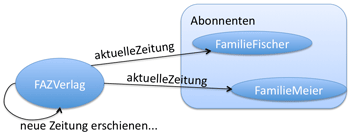
\includegraphics[scale=1]{figure/Observer/einleitungW}} 
			\captionof{figure}{FAZVerlag Problem} 			
		\label{pic:einleitungW}
	\end{center}

	Der FAZ-Verlag versendet die jeweils aktuelle Zeitung an seine Abonnenten Familie Fischer und Meier. \\
	Bei jeder neuen Zeitung soll eine Auslieferung erfolgen.\\ \\
	
	Nachfolgend istl der Sachverhalt als Klassendiagramm dargestellt:

	\begin{center}
		\fbox{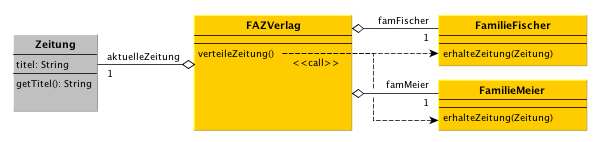
\includegraphics[scale=0.8]{figure/Observer/einleitungI-kl}}
			\captionof{figure}{Klassendiagram FAZVerlag Problem} 			
		\label{pic:einleitungI-kl}
	\end{center}

	FAZVerlag hat von jedem Abonnenten ein Objekt und ruft einzeln die Funktion erhalteZeitung(Zeitung) auf.\\
	\subsection{Java Implementierung}
		Eine schnelle sehr unsaubere L�sung ist hier nachfolgend in Java implementiert:\\

		\begin{lstlisting} [caption={Beispiel Java}\label{lst: Smalltalk_bsp},captionpos=t] 
		public class FAZVerlag { 

			private Zeitung aktuelleZeitung; 
			private FamilieFischer famFischer; 
			private FamilieMeier famMeier; 

			//Sobald eine neue Ausgabe existiert
			public void verteileZeitung() { 
			        famFischer.erhalteZeitung(aktuelleZeitung); 
			        famMeier.erhalteZeitung(aktuelleZeitung); 
			} 
		} 
		\end{lstlisting}


	\subsection{Nachteile}
		\begin{itemize}
			\item{Enge Verbindung zwischen FAZVerlag und Abonnenten}
			\item{Erweiterbarkeit eingeschr�nkt}
			\item{Abonnement bestellen oder abbestellen w�hrend der Laufzeit nicht m�glich.}	
		\end{itemize}

\section{L�sung}

	\begin{center}
		\fbox{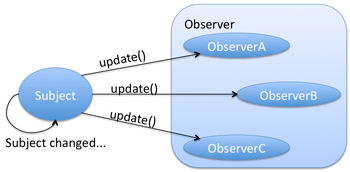
\includegraphics[scale=1]{figure/Observer/observer-def-schema}} 
			\captionof{figure}{Observer Pattern Schema} 			
		\label{pic:observer-def-schema}
	\end{center}

	\begin{center}
		\fbox{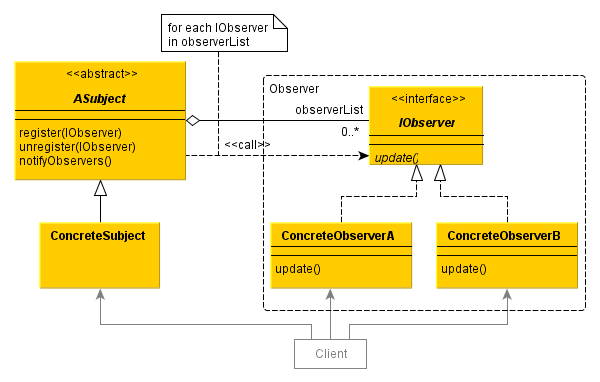
\includegraphics[scale=0.7]{figure/Observer/observer-def-kl}}
			\captionof{figure}{Observer Pattern Klassendiagramm} 			
		\label{pic:observer-def-kl}
	\end{center}



\section{Beispiel}
	\begin{center}
		\fbox{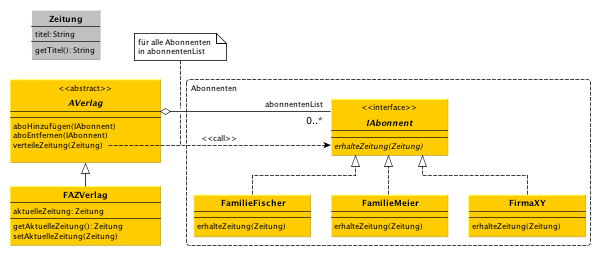
\includegraphics[scale=0.7]{figure/Observer/einleitungV-kl}} 
			\captionof{figure}{Observer Pattern FAZVerlag} 		
		\label{pic:einleitungV-kl}
	\end{center}
